\chapter{Physics Background} \label{ch:physBKGD}
%\newpage
%\section{Introduction}

%The Standard Model of particle physics is described briefly. This theory describes the interactions between subatomic particles. Luminosity, the relevant metric in particle physics experiments as the measure of amount of particle interactions is also described briefly.

%It is the preeminent theory describing the behavior of subatomic particles, and it is the result of generations of experimental observations and theoretical interpretations. 

%Introduction about the chapter.

\section {Standard Model of Particle Physics} \label{sec:stdModel}

The standard model (SM) of particle physics describes the interaction between elementary particles through electromagnetic, weak, and strong forces via the exchange of force mediator particles. This model unifies theories on electromagnetic and weak interactions as published in 1961 [ref Sheldon Glashow], with the addition of Higgs mechanism in 1967 by [Steven Weinberg and Abdus Salam]. This theory successfully explained the experimental observations in the past, as shown in Figure \ref{fig:vstime}, and continues to provide avenues to probe the theory further. 



\begin{figure}[htbp!]
\centering
  \includegraphics[width=0.7\textwidth]%
%    {figures/instrument/25ns_fill_scheme.png}% picture filename
%  {figures/model/Standard_Model_of_Elementary_Particles.svg.png}
  {figures/intro/Standard_Model_of_Elementary_Particles_modified_version}
	\captionsetup{format=hang}
  \caption{The standard model of particle physics with three generations
of matter fermions, gauge bosons and a Higgs boson. Figure taken from \cite{wiki:SMfigure}}
	\label{fig:particles}
\end{figure}



%\subsection {Elementary Particles}
According to the SM, matter consists of particles of spin 1/2 known as fermions each of which has its own antiparticle of opposite spin. These particles are treated as excitations of fields, and the forces are treated as interactions between these excitations. The interactions happen via exchange of various vector bosons, which are the particles with spin 1. There are two groups of fermions: that interact electromagnetically and weakly. The Leptons--electron, muon, tau, and their partner neutrinos only experience the electroweak force. The quarks--up, down, strange, charm, bottom, top experience both the electroweak force and the strong force. Higgs boson, with spin 0, generates mass of particles. As the unification in the SM a priori only is valid with massless particles, Higgs mechanism describes the process by which particles require mass. 


The particle content of the SM is summarized in Figure \ref{fig:particles}. Protons and neutrons that make up most of the matter around us are composed of quarks.  

\begin{table}
\begin{center}
    \begin{tabular}{| l | l | l | l |}
    \hline
    {\bf Interaction} & {\bf Strength} & {\bf Mediator} \\ \hline
    Strong & 10  & Gluon \\ \hline
    Electromagnetic & $10^{-2}$  & Photon \\ \hline
    Weak & $10^{-3}$ &   W and Z Bosons\\ \hline
    Gravitation & $10^{-42}$  & Graviton \\
    \hline
    \end{tabular}
	\captionsetup{format=hang}    
     \caption{Rough order of the interaction strengths and the mediators for interactions.}

\end{center}
\end{table}



Despite its successes in describing particle interactions at energies accessible with particle accelerators, the SM is not a complete theory of the universe. This is among the strongest reason to search for physics beyond the SM. During future data-taking periods LHC hopes to push our understanding forward by observing new generations of particles and particle interaction rates that deviate from SM predictions.

%Neutrinos, which have very small mass, are electrically neutral and thus only participate in weak interactions. Despite its successes in describing particles physics across huge mass scale, Standard Model it is not a complete theory of the universe. This is among the strongest reasons to keep looking for physics beyond SM. The future data-taking periods of LHC hopes to push our understanding forward.


%CERN\footnote{European Organization for Nuclear Research}

%\begin{figure}[htbp!]
%\begin{center}
%  \includegraphics[width=1.0\textwidth]%
%%    {figures/instrument/25ns_fill_scheme.png}% picture filename
%%  {figures/model/Standard_Model_of_Elementary_Particles.svg.png}
%  {figures/intro/discoveries.pdf}
%	\captionsetup{format=hang}
%  \caption{The discoveries of fundamental particles of the Standard Model vs time \cite{Thesis:Tuna}}
%  \label{fig:vstime}
%\end{center}
%
%\end{figure}






\section{Luminosity}
%\subsection{Introduction}

The quantity that measures the ability of a particle collider to produce the required number of interactions is called the luminosity $\mathcal{L}$. Its precise knowledge is important since for many cross-sections measurements the uncertainty factor on the luminosity dominates the final result. Luminosity is the proportionality factor between the number of events per second $R(t)$ at a given time $t$ and its production cross-section $\sigma_{P}$ for a process:

\begin{equation} \label{eq:rate}
R(t) = \mathcal{L}(t) \cdot \sigma_{P}
\end{equation}

This defines the so-called instantaneous luminosity commenly measured in units of cm$^{-2}$ s$^{-1}$. Typically running conditions vary with time $t$. Therefore, the luminosity of a collider also has a time dependence that needs to be carefully measured to arrive at integrated luminosity for a given data taking period which is given as:

\begin{equation} \label{eq:instLumi}
\mathcal{L}_{int} = \int \mathcal{L}(t) dt
\end{equation}
and measured in units of b$^{-1}$\footnote{1 barn = $10^{-28}$ cm$^2$}. The delivered integrated luminosity, which refers to the integrated luminosity which the machine has delivered to an experiment, and recorded integrated luminosity, which refers to the amount of data that has actually been stored to disk by the experiments typically differ and hence an independent measurement by the experiment is necessary.

As $\mathcal{L}$ is process-independent it is possible to measure the luminosity with any process whose cross-section is known. For a precise luminosity determination, however, it is essential that the process has precise theoretical predictions and at the same time that its rate can be accurately measured, i.e. enough, signal events are produced and reconstructed in a limited time interval. The production of $Z^{0}$ bosons $(pp \rightarrow Z^{0} X) $ that decay into leptons, particularly muons $(Z^{0} \rightarrow \mu^{+} \mu^{-})$, is such a "standard candle process", because the leptons can be well identified and theoretical prediction of the cross section has only a few percent relative uncertainty. The cross-section of $Z^{0}$ production is large enough and there are almost no fake signals.


% Colliding Beams
\begin{figure}
\centering
\begin{tikzpicture}[scale=1.25]
%    \draw [red] (0,0) ellipse (2cm and 0.25cm);
    \draw [->, red] (-1,0.5) -- (1,0.5);
    \node (draw) at (0,1) {$n_{1}$};% \rho_{1}(x,y,s;-s_{0})$};
%  \node [cylinder, gray!50, rotate=0, draw,
  \node [cylinder, red, rotate=0, draw,
    minimum height=3cm, minimum width=1cm] at (0,0) {};

    \filldraw (2.5,0) circle (1pt);

  \node [cylinder, blue, rotate=180, draw,
    minimum height=3cm, minimum width=1cm] at (5,0) {};

    \draw [->, blue] (6,0.5) -- (4,0.5);
    \node (draw) at (5,1) {$n_{2}$};% \rho_{2}(x,y,s;s_{0})$};

    \draw[->] (-3,0) -- (7,0) node[right] {$z$};


\node[align=center] at (2.5,-1) (ori) {$A_{eff}$};
\draw [->] (2.5,-0.9) --(1.1,0);

\end{tikzpicture}
\caption{Two colliding proton beam bunches with idealized shape} \label{fig:collBeams}
\end{figure}


The instantaneous luminosity can be extracted from certain beam parameters. A simplified case for a head-on collision of two bunches is shown in Figure \ref{fig:collBeams}. The luminosity can be expressed in terms of geometry and the number of particles in each of the two colliding beam bunches $n_{1(2)}$:

\begin{equation} \label{eq:intLumi}
\mathcal{L} = \frac{n_{1} n_{2} f}{A_{eff}},
\end{equation}

\noindent
with $f$ the collision frequency. Beam parameters for the LHC are listed in Table \ref{tbl:beamParam}. Of the possible 3564 bunches only $n_{b} = 2808$ are filled reducing the peak luminosity accordingly. The beam current $I_{1(2)}$ is given in terms of the charge of the beam particle $e$ and the collision frequency $f$ as $I_{i} = e_{i} f n_{i}$. Hence, one obtains

\begin{equation}
\mathcal{L}_{int} = \frac{I_{1} I_{2}}{e^{2} f A_{eff}}
\end{equation}

\begin{figure}
\begin{center}
  \includegraphics[width=1.0\textwidth]%
  {figures/intro/crosssections.pdf}
	\captionsetup{format=hang}
  \caption{The cross sections and expected production rates at the LHC and the Tevatron.}
  \label{fig:crossSection}
\end{center}

\end{figure}


With a nominal instantaneous luminosity of $\mathcal{L} = 10^{34}$cm$^{-2}$s$^{-1} (= 10$ nb$^{-1}$ s$^{-1})$ and a Higgs production cross section of $\sigma \simeq 0.1 $nb one expects about 1 Higgs per second. Figure \ref{fig:crossSection} shows the cross sections for several processes at a 10 times lower  nominal luminosity that has been achieved so far with the LHC. At this luminosity also about 100 $Z^{0}$ particles are produced per second. Only 3.4 \% of $Z^{0}$'s decay into a muon pair resulting in about 3 $Z^{0}$ particles per second that are potentially detected and reconstructed with CMS.


\begin{table}[htp]
\begin{center}
\begin{tabular}{|l|c|c|}
\hline
{\bf Beam Parameter} & {\bf Unit} & {\bf Value} \\ \hline
Proton Energy & [GeV] & 6500 \\ \hline
Stored energy per beam & [MJ] & 363 \\ \hline
Number of particles per bunch $n_{i}$ & & $1.15 \times 10^{11}$ \\ \hline
Number of bunches $n_{b}$ & & 2808 \\ \hline
Bunch collision frequency $f$ & MHz & 40 \\ \hline
Circulating beam current & [A] & 0.584 \\ \hline
Transverse beam size ($\sigma_{x,y}$) & $\mu m$ & 16.7 \\ \hline
RMS bunch length ($\sigma_{z}$ & cm & 7.55 \\ \hline
Geometric luminosity reduction factor F & & 0.836 \\ \hline
Peak luminosity in IP1 and IP5 & [$cm^{-2} sec^{-1}$] & $10^{34}$ \\ \hline \hline

\end{tabular}
\end{center}
    \captionsetup{format=hang}
     \caption{LHC beam parameters relevant for the peak luminosity \cite{fill-schemes}}
    \label{tbl:beamParam}
\end{table}%


Assuming that the transverse profile of the two bunches distribute identically and that the profiles do not change along the bunch a good approximation is a Gaussian profile for the beam transverse distribution in $x$ and $y$, each characterized with a standard deviation $\sigma_{x}$ and $\sigma_{y}$, respectively. In this case $A_{eff} = 4 \pi \sigma_{x} \sigma_{y}$. It implies that the profiles in $x$ and $y$ direction are not correlated.


The two beams at the LHC cross each other under an angle of $\theta_{C} = 285 \mu $ rad to direct the beams after collision into their respective vacuum pipe and to avoid multiple unwanted interactions. Figure \ref{fig:rotBeams} shows a schematic illustration of the beam crossing. It also shows a change in the profile along the beam width. The correct evaluation of the effective beam size is obtained from an overlap integral of beam density distribution functions in all three coordinates \cite{lumiConcepts}. For small angles, Gaussian profiles and $\sigma_{x} \simeq \sigma_{y}$ in good approximation this results in the so called geometric luminosity reduction factor F, given as


\begin{equation} \label{eq:lumiAcc}
F = \left(  \sqrt{1 + \left( \frac{\theta_{c} \sigma_{z}}{2 \sigma^{*}} \right ) ^{2}}  \right) ^{-1}
\end{equation}

that multiplies eq. \ref{eq:intLumi}.

% Colliding Beams at some angle

\begin{figure}[h]
\centering
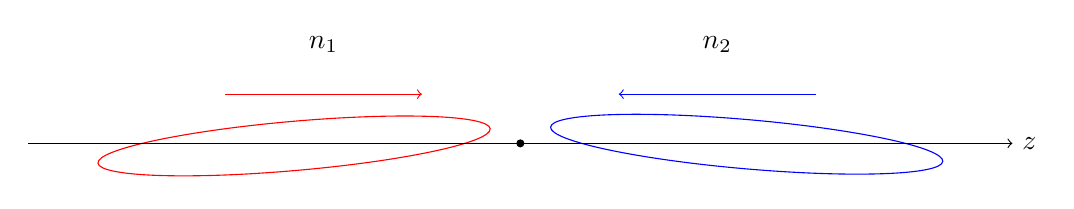
\begin{tikzpicture}[scale=1.25]
    \draw [red,rotate around={5:(0,0)}] (-0.3,0) ellipse (2cm and 0.25cm);
    \draw [->, red] (-1,0.5) -- (1,0.5);
    \node (draw) at (0,1) {$n_{1}$};% \rho_{1}(x,y,s;-s_{0})$};

   \filldraw (2,0) circle (1pt);

    \draw [blue,rotate around={-5:(4.2,0)}] (4.3,0) ellipse (2cm and 0.25cm);
    \draw [->, blue] (5,0.5) -- (3,0.5);
    \node (draw) at (4,1) {$n_{2}$};%\rho_{2}(x,y,s;s_{0})$};

%    \draw [->] (-4,0) -- (0,0) -- (1,0) -- (8,0);
    \draw[->] (-3,0) -- (7,0) node[right] {$z$};

\end{tikzpicture}
\caption{Two proton bunches with more realistic profile colliding at an angle} \label{fig:rotBeams}
\end{figure}


In practice, however, there are complications: beams do not factorize as the profile changes over the length of the bunch and bunches do not collide exactly head-on but with offsets. Imperfections in the beam steering lead to widening of the beam profile and therefore a reduced luminosity. So far also a uniform population of the beam bunches is assumed while in reality the actual fill pattern can vary. The LHC provides measurements of beam currents and beam profiles along the LHC accelerator but not in the vicinity of the interaction points. Furthermore, the beam parameters and conditions change over the time period of a LHC fill. To arrive at the best time-integrated luminosity the time integral has to be taken over time intervals short enough to measure significant variations and exclude dead times. Typically the beam intensity decays exponentially with time resulting in a similar reduction in the instantaneous luminosity. The effective mean lifetime of the luminosity is further reduced by the increase of the transverse and longitudinal beam size over time. To reduce uncertainties due to extrapolation from beam parameter measurements the CMS experiment has to measure the relative luminosity with dedicated detectors and calibrate them with standard candle processes or dedicated calibration runs of the LHC. 




\section {Luminosity Calibration} \label{sec:lumiCalibration}
One can obtain the absolute luminosity directly from beam parameters according to Eq.~\ref{eq:instLumi}, 
without the a priori knowledge of any physics cross section.
The revolution frequency $f$ is well known and the number of particles
$n_{1(2)}$ can be measured by dedicated beam charge monitors.
In contrast, the transverse area of beam overlap $A_{eff}$ is difficult to determine.
Different monitors such as wire scanners or synchrotron light monitors can sample the beam
profile but not close to the collision points and extrapolations lack precision.
In the year 1968 Simon van der Meer proposed a method to measure $A_{eff}$~\cite{vanderMeer:296752}, now  known as van der Meer- (vdM-) or beam separation-scan.

Simon van der Meer proposed that it is possible to measure the profile of colliding beams
by observing the counting rate $R$ in a particle counting system, while scanning the two
beams vertically across each other. One of the two beams is displaced vertically with respect 
to the other one, and the counting rate in the monitor is plotted versus displacement.
A bell-shaped curve will result with its maximum at zero displacement, then independent  of beam shape $A_{eff}$ is equal to the area under this curve,
divided by the ordinate for zero displacement~\cite{vanderMeer:296752}.
%  S. van der Meer, Calibration of the effective beam height in the ISR,
%  CERN-ISR-PO-68-31, 1968.
%
At the LHC the measured counting rate
depends on both horizontal and vertical beam sizes. The main assumption is that the 
density distributions of particles in bunches can be factorized, and two scans along
the transverse planes are sufficient. If one assumes that the beam density functions 
are uncorrelated one can write for the counting rate $R$ as function of displacement
in $x$ and $y$, $\delta x$ and $\delta y$, respectively:
\begin{equation}
R(\delta x;\delta y) = R_x(\delta x) R_y(\delta y)
\end{equation}
By scanning the two transverse planes, one obtains a direct measurement of the transverse
effective beam sizes and therefore of the effective area $A_{eff}$:
\begin{equation}
A_{eff} = \frac{\int R_x(\delta x) d\delta x}{R_x(0)} \frac{\int R_y(\delta y) d\delta y}{R_y(0)}
\end{equation}
The convoluted transverse width per scan direction of the two beams can be written as:
\begin{equation}
\Sigma_x = \sqrt{\sigma_{1x}^2+\sigma_{2x}^2} = \frac{1}{\sqrt{2\pi}}\frac{\int R_x(\delta x) d\delta x}{R_x(0)} 
\end{equation}  
and the same expression for $\Sigma_y$ in $y$ direction. The luminosity Eq.~\ref{eq:instLumi} becomes:
\begin{equation}
{\cal L}_{\mbox{int}} = \frac{n_1 n_2 f}{2\pi \Sigma_x \Sigma_y} 
\end{equation}
In case of a crossing angle, the vdM scan measures directly the correct effective
beam size, including the effect of a crossing-angle for scans performed exactly in the
crossing plane~\cite{White:1308187}
% S. M. White, Determination of the Absolute Luminosity at the LHC. PhD thesis,
% Orsay, Universite Paris-Sud 11, Orsay, 2010. oai:cds.cern.ch:1308187.
%
Figure~\ref{fig:Scan1Fits} shows the rate of particle tracks as measured with the PLT versus
the separation in the beam in $x$ direction. The data points have been fit to a Gaussian 
function. A refined fit uses two Gaussian functions to achieve an improved description
of the tails in the distribution.

The CMS collaboration uses the PLT detector to measure and monitor the relative luminosity. 
Once calibrated, one can extrapolate the absolute luminosity measurement of the 
vdM scan to any other luminosity scenario. With $R_{\mbox{inel}}$ to be the rate of inelastic 
$pp$ events, $\sigma_{\mbox{inel}}$ the $pp$ inelastic cross-section, $f$ the revolution frequency 
of the bunches, and $\mu$ the average number of $pp$-collisions per bunch-crossing:
\begin{equation}
{\cal L}_{\mbox{int}} = \frac{R_{\mbox{inel}}}{\sigma_{\mbox{inel}}} = \frac{\mu f}{\sigma_{\mbox{inel}}}
\end{equation}
The PLT detector with limited acceptance times detection efficiency $\omega$ will only see a subset of the events:
\begin{equation}
{\cal L}_{\mbox{int}} = \frac{\omega \mu f}{\omega \sigma_{\mbox{inel}}} = \frac{\mu_{\mbox{vis}} f}{\sigma_{\mbox{vis}}}
\end{equation}
The index $\mbox{vis}$ stands for visible value. Hence, the $\mu_{\mbox{vis}}$ can be measured and
${\sigma_{\mbox{vis}}} = {\sigma_{\mbox{inel}}}$ is practically the calibration constant to obtain the absolute luminosity.
In general, this equation is valid only in the case of a linear response of the detector with 
respect to $\mu$. Otherwise corrections for the non-linearity must be taken into account.


\section {Luminosity Measurement} \label{sec:lumiMeasurement}
The PLT detector consists of two symmetric detector arms placed on each side of the CMS interaction point (IP5).
Each side is further divided into eight telescopes with each treated as separate readout channel. Particles passing
through one of these telescopes are counted as hit if their charge signals in all three detectors of the
telescope are simultaneously above threshold (Fast-OR). A bunch crossing is counted as an event when there is at least 
one hit. The typical rate $\mu$ per bunch crossing in 2015 was 1 hit on each side respective
a detector occupancy of about 0.15/BCX. Particles not originating from bunch collisions but rather
collision in the beam gas and with beam halo particles result in a miscount of the luminosity and
are subtracted statistically after a detailed analysis of their relative contribution.The relative
contribution from such background was at most 7\% in 2015. The analysis is described in detail in ~\cite{PLT:AN-16-002_v3}.
The luminosity is determined by event-counting. A disadvantage of this method is that one is
limited to measure either any hit or no-hit event which at high $\mu$ results in the event probability
approaching one. Then every bunch crossing will be counted as an event and the method does
not work anymore (is saturated). 

One can derive the probability for multi-interaction events making the assumption that 
the number of $pp$ interactions during a bunch crossing follows a Poisson statistics the following:
\begin{equation}
P_{\mu}(n) = \sum_{n=0}^{\infty} \frac{\mu^n e^{-\mu}}{n!}
\end{equation}
where $P_\mu(n)$ is the probability to have $n$ interactions in a bunch crossing when the average 
number of interactions is $\mu$. Furthermore, the probability to detect a single interaction $\omega$ 
(efficiency $\times$ acceptance of the PLT Fast-OR) is assumed not to change when several events in the same 
bunch crossing happen. This effect is expected to be negligible for occupancies of significantly less than 1 per 
bunch crossing per channel. The probability for {\em not} detecting a bunch crossing
that has $n$ interactions is given as:
\begin{equation}
P_0(n) = (1 - \omega)^n 
\end{equation}
With $n$ distributed according to a Poissonian the probability to measure $\mu$ interactions
when the average number is zero is:
\begin{equation}
P_0(\mu) = \sum_{n=0}^{\infty} (1 - \omega)^n \cdot P_{\mu}(n)
\end{equation}
and using the expansion one obtains:
\begin{equation}
P_0(\mu) = e^{-\omega \mu} = e^{-\mu_{vis}}
\end{equation} 
With $N_{OR}$ the number of Fast-OR events in a given time interval, and $N_{BCX}$ the
corresponding number of bunch crossings, the probability to observe a Fast-OR $P_{OR}$ 
in a given bunch crossing is:
\begin{equation}
P_{OR}(\mu) = \frac{N_{OR}}{N_{BCX}} = 1 - P_0(\mu) = 1 - e^{\mu_{vis}}
\end{equation} 
From the latter two one obtains an expression for $\mu_{vis}$:
\begin{equation}
\mu_{vis} = - ln(1 - P_{OR}(\mu))
\end{equation}
 

The PLT obtains $\mu_{vis}$ per telescope for each of the potential 3564 bunch positions  
for 4096 orbits of the LHC beam, also called nibble corresponding to 0.365 ms.
Instead of counting $N_{OR}$ the fraction $f_0 = (1 - N_{OR}/N_{BCX})$ of no triple coincidences
in that interval is measured. This has the advantage that the multiplicity of tracks does not have
to be resolved and readout only has to register signal or no signal, 0 or 1, respectively.
This is the digital mode and the method is called zero-counting. The mean number of tracks per collision 
is then given as $\mu_{vis} = -\ln ( f_0 )$.
The $\mu_{vis}$ is summed over all bunch crossings and averaged over all telescopes
and translated into the luminosity with the calibration constant $\sigma_{vis}$.
Recently, instead of averaging over telescopes, the luminosity is provided on a per-telescope basis.




